\subsection{Conception}
	\begin{frame}
		\frametitle{Organisation des classes}
		\begin{center}
			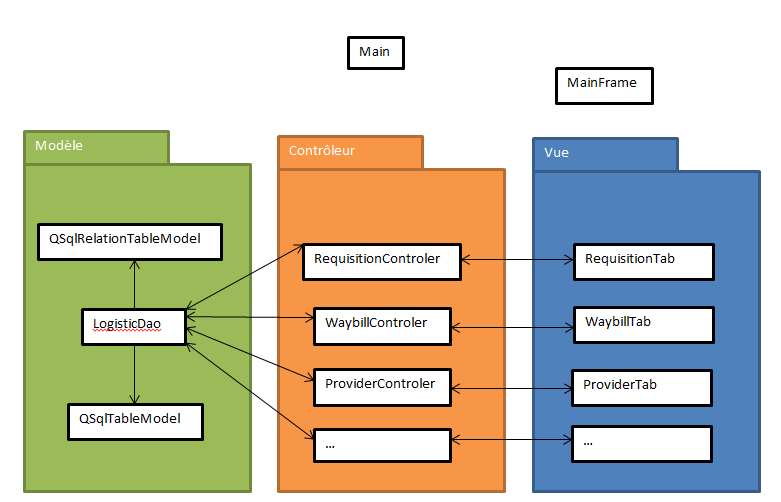
\includegraphics[scale=0.45]{Images/OrganisationClasses}
		\end{center}
	\end{frame}
	\begin{frame}
		\frametitle{Organisation des classes}
		\begin{figure}[htbp]
			\centering
			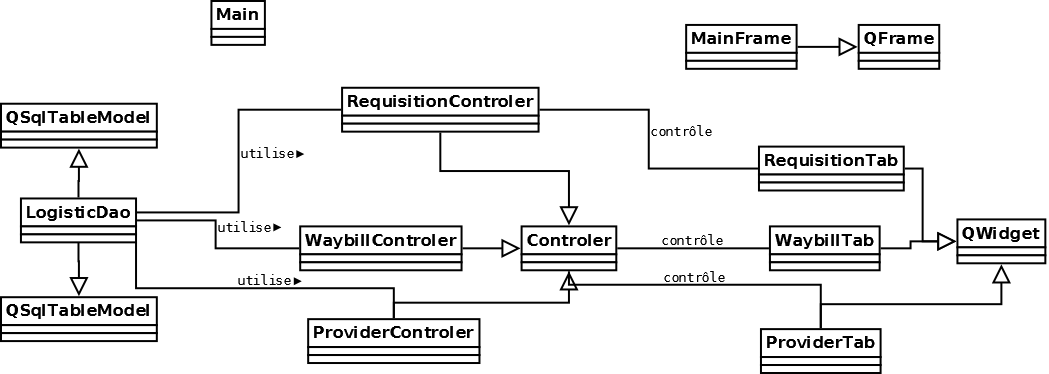
\includegraphics[scale=0.2]{Images/DiagrammeClasses}
			\caption{Diagramme des classes}
		\end{figure}
	\end{frame}
\subsection{Réalisation}
	\begin{frame}
		\frametitle{Interface graphique}
		\begin{figure}[htbp]
			\centering
			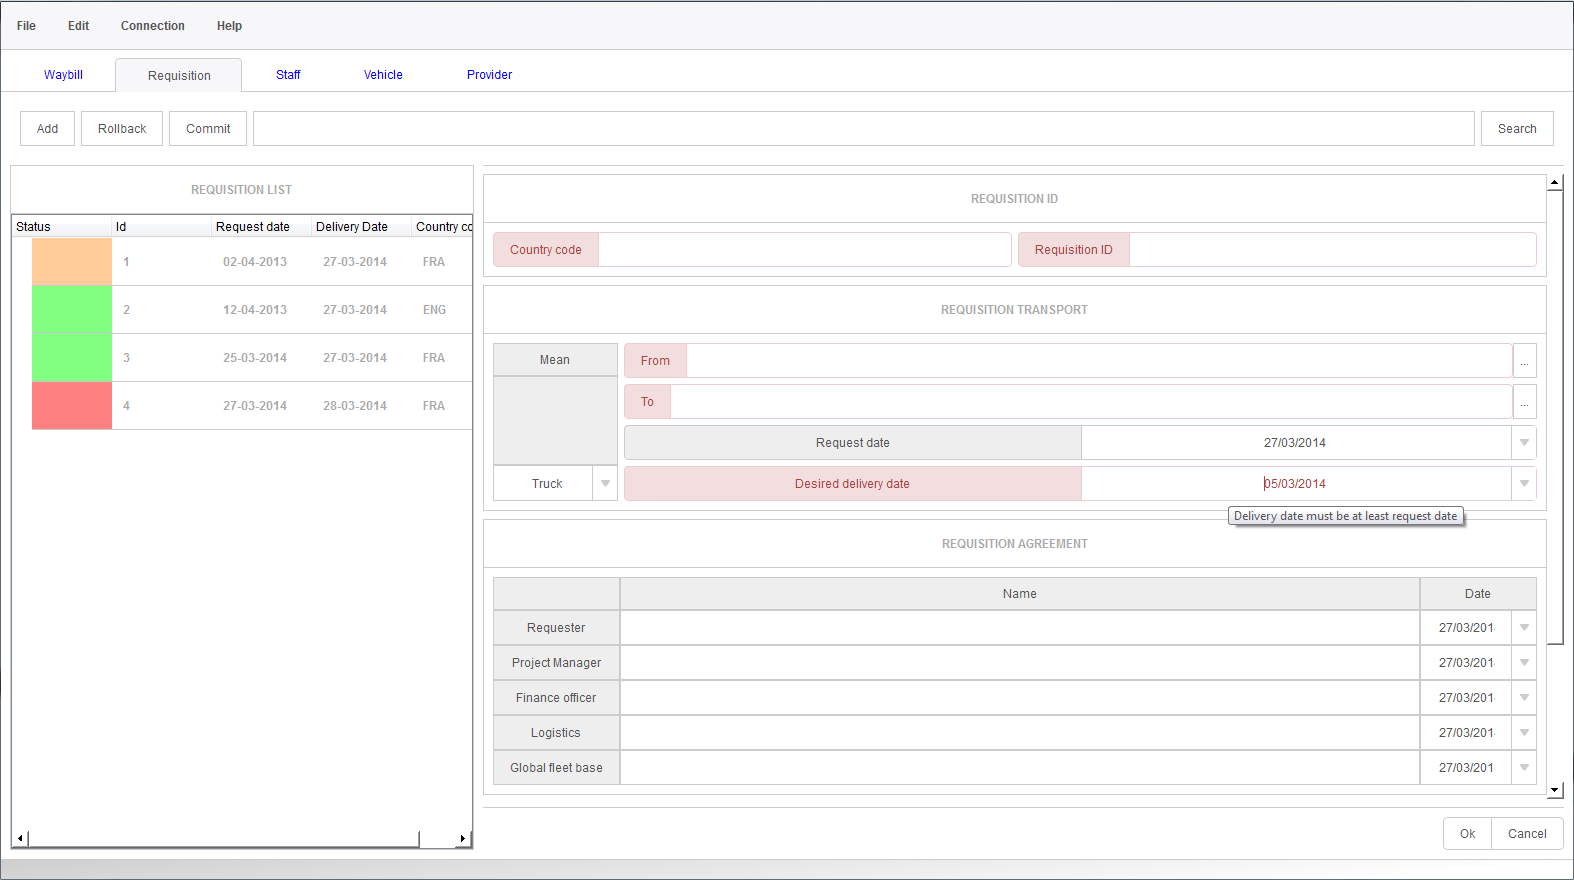
\includegraphics[scale=0.24]{Images/Interface}
			\caption{Interface graphique du TMS}
		\end{figure}
	\end{frame}
	\begin{frame}		
		\frametitle{Avancement de la réalisation}
		\begin{block}{\textbf{Ce qui est fait}}
			\begin{itemize}
				\item Mise en place de la couche DAO
				\item Réalisation de l'interface graphique (Frames, css)
				\item Mise en place de validateurs (requisition, waybill)
				\item Ajout/modification de réquisitions
			\end{itemize}
		\end{block}
	\end{frame}
	\begin{frame}	
		\frametitle{Avancement de la réalisation}
		\begin{block}{\textbf{Ce qui reste à faire}}
			\begin{itemize}
				\item Mise en place des validateurs dans les autres onglets
				\item Ajout/modification de waybill, conducteurs, prestataires
				\item Gestion de la synchronisation
				\item Gestion des imports/exports de données
			\end{itemize}
		\end{block}
	\end{frame}